% Appendix X

\chapter{User Defined Function}

\definecolor{codegreen}{rgb}{0,0.6,0}
\definecolor{codegray}{rgb}{0.5,0.5,0.5}
\definecolor{codepurple}{rgb}{0.58,0,0.82}
\definecolor{backcolour}{rgb}{0.95,0.95,0.92}

\lstdefinestyle{mystyle}{
	backgroundcolor=\color{backcolour},   
	commentstyle=\color{codegreen},
	keywordstyle=\color{magenta},
	numberstyle=\tiny\color{codegray},
	stringstyle=\color{codepurple},
	basicstyle=\footnotesize,
	breakatwhitespace=false,         
	breaklines=true,                 
	captionpos=b,                    
	keepspaces=true,                 
	numbers=left,                    
	numbersep=5pt,                  
	showspaces=false,                
	showstringspaces=false,
	showtabs=false,                  
	tabsize=2
}

\lstset{style=mystyle}

In seguito sono state definite le User Defined Function (da qui in avanti indicate con l’acronimo UDF), che eseguono automaticamente il calcolo del valore di exposure per le stazioni ferroviarie. Tali UDF sono state realizzate nel linguaggio PL/pgSQL offerto da PostgreSQL, sfruttando le funzioni fornite dall’estensione spaziale PostGIS.

\section{UDF per le stazioni}
E' stato realizzato uno script Python, \textit{HotSpotCalculator}, in grado di collegarsi al database ed eseguire la UDF  \textit{\_\_exposure(id\_building)}. Quest'ultima è la funzione fondamentale in quanto richiama sequenzialmente tutte le UDF necessarie per il calcolo dell'exposure di una stazione. L'ultima UDF eseguita, ovvero la \textit{\_\_contributionoflandslide(id\_building,l)} inserisce il risultato nella tabella \textit{exposure\_station} (Figura \ref{diagramma_algoritmo}). 

\begin{figure}[h]
	\centering
	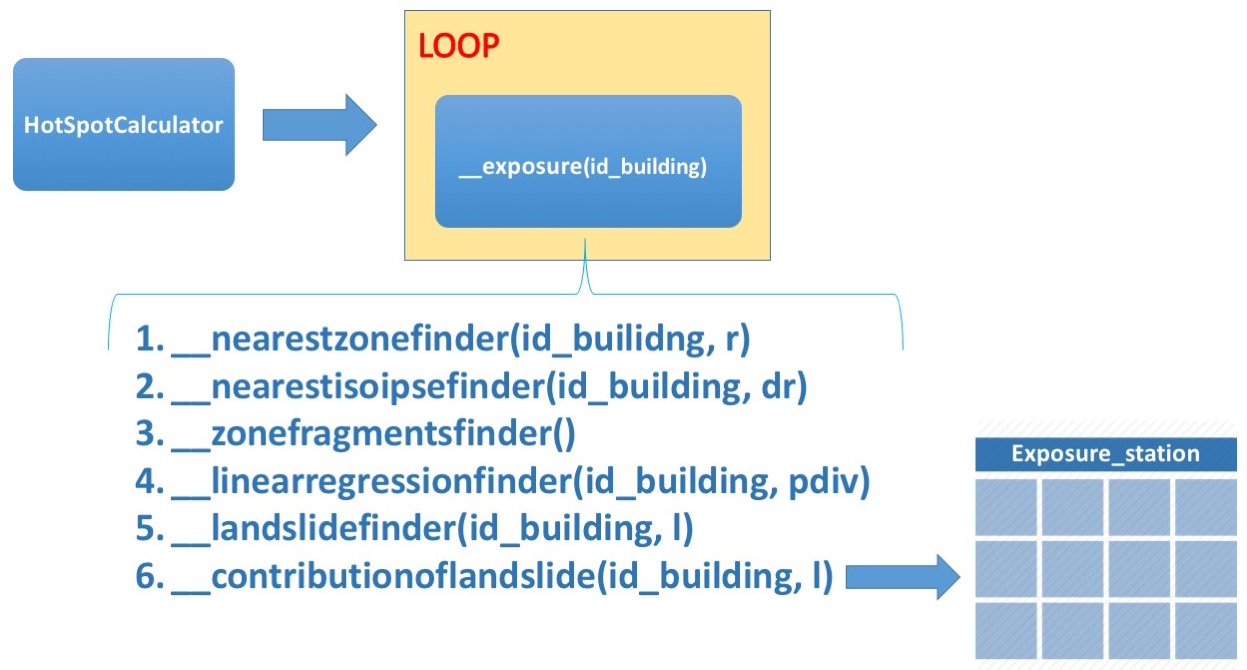
\includegraphics[width=0.9\textwidth]{images/algorithm}
	\caption{Diagramma del funzionamento dell'algoritmo realizzato.}
	\label{diagramma_algoritmo}
\end{figure}

Lo script Python itera \textit{\_\_exposure} per tutte le stazioni. Inoltre stima il tempo necessario e stampa a video il numero di exposure calcolate.

\subsection{\_\_exposure}
\textbf{INPUT}: \textit{id\_building} corrisponde all'ID del $b_i$ \newline
\textbf{OUTPUT}: \textit{void}. \newline
\textbf{COMMENTO}: Rappresenta la main function. Esegue in successione sulla $b_i$ le UDF necessarie al calcolo dell'exposure. Crea la tabella exposure\_stations dove verranno salvato il valore dell'exposure.   

\begin{lstlisting}[language=SQL]
create or REPLACE function "__exposure"(id_building integer) returns void
LANGUAGE plpgsql
AS $$
DECLARE
	point RECORD;
	exposure RECORD;
BEGIN

	DROP TABLE IF EXISTS nearestzones;
	DROP TABLE IF EXISTS nearestisoipses;
	DROP TABLE IF EXISTS zonefragments;
	DROP TABLE IF EXISTS linearregression;
	DROP TABLE IF EXISTS landslide;
	DROP TABLE IF EXISTS landslidezones;
	DROP TABLE IF EXISTS exposure_stations;

	CREATE TABLE IF NOT EXISTS exposure_stations(
		id SERIAL PRIMARY KEY ,
		Building_gid INTEGER,
		name varchar,
		geom geometry,
		exposure FLOAT
	);

	DROP TABLE IF EXISTS points;
	CREATE TABLE points AS (SELECT * FROM railway_stations);


	FOR point IN SELECT * FROM points where gid=id_building LOOP
		PERFORM __nearestzonefinder(point.gid,800);
		PERFORM __nearestisoipsefinder(point.gid,850);
		PERFORM __zonefragmentsfinder();
		PERFORM __linearregressionfinder(point.gid,2.5);
		PERFORM __landslidefinder(point.gid,50);
		PERFORM __contributionoflandslide(point.gid,50);

		SELECT * FROM exposure LIMIT 1 INTO exposure;
		INSERT INTO exposure_stations (Building_gid, name, geom, exposure) VALUES (exposure.id, exposure.name, exposure.geom, exposure.exposure);
	END LOOP;

	PERFORM __cleartables();
END;
$$;
\end{lstlisting}

\subsection{\_\_NearestZoneFinder}
\textbf{INPUT}: 
\begin{enumerate}
	\item \textit{id\_building} è l'ID del $b_i$;
	\item \textit{r} è il raggio della $HazardArea_i$.
\end{enumerate}
\textbf{OUTPUT}: \textit{void}. \newline
\textbf{COMMENTO}: trova tutte le zone che si trovano all'interno della $HazardArea_i$ di $b_i$. I risultati vengo salvati all'interno della tabella NearestZones.

\begin{lstlisting}[language=SQL]
CREATE OR REPLACE FUNCTION __NearestZoneFinder (id_building integer, r integer) RETURNS void
LANGUAGE plpgsql
AS $$
DECLARE
	building RECORD;
	zone RECORD;
	hazardArea geometry;
BEGIN

	CREATE TEMP TABLE hotspottmp ( id serial PRIMARY KEY, id_station INTEGER, geom Geometry, szk FLOAT  ) ON COMMIT DROP;
	SELECT * INTO building FROM points where gid = id_building;

	hazardArea := (SELECT ST_Buffer(building.geom, r));

	FOR zone IN SELECT * FROM dataset LOOP
		IF ST_Intersects(hazardArea, zone.geom) THEN
			INSERT INTO hotspottmp (id_station, geom, szk) VALUES(building.gid, ST_Intersection(hazardArea, zone.geom), zone.szk );
		END IF;
	END LOOP;
	CREATE TABLE NearestZones AS SELECT * FROM hotspottmp;
	DROP TABLE hotspottmp;
END;
$$
\end{lstlisting}

\subsection{\_\_NearestIsoipseFinder}

\textbf{INPUT}: 
\begin{enumerate}
	\item \textit{id\_building} è l'ID del $b_i$;
	\item \textit{dr} il raggio leggermente più grande rispetto all'$HazardArea_i$.
\end{enumerate}
\textbf{OUTPUT}: \textit{void}. \newline
\textbf{COMMENTO}: trova tutte le $ni_{i,o}$ e le inserisce nella tabella \textit{NearestIsoipses}. L'$HazardArea_i$ ha, in questo unico caso, un raggio leggermente più grande. Ciò è necessario per ottenere che le $ni_{i,o}$ escano dal perimetro delle $nz_{i,j}$ così che la UDF successiva (\textit{\_\_ZoneFragmentsFinder}) esegua correttamente la funzione ST\_SPLIT(). 

\begin{lstlisting}[language=SQL]
CREATE OR REPLACE FUNCTION __NearestIsoipseFinder (id_building integer, dr integer) RETURNS void
LANGUAGE plpgsql
AS $$
DECLARE
	building RECORD;
	hazardArea geometry;
BEGIN
	
	CREATE TEMP TABLE tempIsoipse (
		id SERIAL PRIMARY KEY ,
		geom GEOMETRY,
		elevation INTEGER
	);
	
	SELECT * INTO building FROM points WHERE gid=id_building;
	hazardArea := (SELECT ST_Buffer(building.geom, dr));
	
	--- intersezione tra hazardArea e Isoipse
	INSERT INTO tempIsoipse (elevation,geom) (SELECT isoipse_abruzzo_25.elevation,st_intersection(isoipse_abruzzo_25.geom,hazardArea) as geom
	FROM isoipse_abruzzo_25 WHERE st_intersects(isoipse_abruzzo_25.geom,hazardArea));
	
	--- estrazione da multilineString a linestring
	
	INSERT INTO tempIsoipse(elevation,geom) (SELECT tempIsoipse.elevation,(st_dump(tempIsoipse.geom)).geom FROM tempIsoipse WHERE st_geometrytype(tempIsoipse.geom) = 'ST_MultiLineString') ;
	INSERT INTO tempIsoipse(elevation,geom) (SELECT tempIsoipse.elevation, st_linemerge(tempIsoipse.geom) FROM tempIsoipse WHERE st_geometrytype(tempIsoipse.geom) = 'ST_MultiLineString');
	DELETE FROM tempIsoipse WHERE st_geometrytype(tempIsoipse.geom) = 'ST_MultiLineString';
	
	CREATE TABLE NearestIsoipses AS SELECT * FROM tempIsoipse;
	
	DROP TABLE tempIsoipse;
END;
$$
\end{lstlisting}

\subsection{\_\_ZoneFragmentsFinder}
\textbf{INPUT}: non ci sono parametri in ingresso. \newline
\textbf{OUTPUT}: \textit{void}. \newline
\textbf{COMMENTO}: suddivide tutti le $nz_{i,j}$ di $b_i$ in zone fragments. I risultati vengono inseriti nella tabella \textit{ZoneFragments}.

\begin{lstlisting}[language=SQL]
CREATE OR REPLACE FUNCTION __ZoneFragmentsFinder () RETURNS void
LANGUAGE plpgsql
AS $$

DECLARE
	NearestZone RECORD;
	PrimaIsoipse RECORD ;
	TempFragment RECORD;
	CurrentIsoipse RECORD;
	zoneCorrente RECORD;

BEGIN

	CREATE TABLE ZoneFragments(
		id SERIAL PRIMARY KEY ,
		geom GEOMETRY,
		id_zone INTEGER
	);

--- Prendo un primo poligono e interseco con le curve di livello (curve risultanti dall'intersezione con il buffer)

	FOR NearestZone IN (SELECT * FROM  nearestzones) LOOP
		CREATE TEMP TABLE TempIsoipses(
			id INTEGER,
			geom GEOMETRY,
			elevation INTEGER
		);
		CREATE TEMP TABLE TempFragments(
			id SERIAL PRIMARY KEY ,
			geom GEOMETRY,
			id_zone INTEGER
		);
		CREATE TEMP TABLE CurrentIsoipses(
			id INTEGER ,
			geom GEOMETRY,
			elevation INTEGER
		);

		SELECT * INTO zoneCorrente FROM nearestzones WHERE id = NearestZone.id;
		INSERT INTO TempIsoipses(id,geom,elevation) (SELECT nearestisoipses.id,(st_dump(st_collectionextract(st_intersection(nearestisoipses.geom,zoneCorrente.geom),2))).geom as geom,nearestisoipses.elevation FROM nearestisoipses);

		--- Prima split (popolamento temp fragment)
		SELECT * INTO PrimaIsoipse FROM (SELECT * FROM nearestisoipses WHERE (SELECT id From TempIsoipses LIMIT 1) = nearestisoipses.id) as prima;
	
		INSERT INTO TempFragments(geom,id_zone) (SELECT (st_dump(st_collectionextract(st_split(zoneCorrente.geom,PrimaIsoipse.geom),3))).geom , zoneCorrente.id);
	
		--- delete isoipse
		DELETE FROM TempIsoipses WHERE TempIsoipses.id = PrimaIsoipse.id;
	
		WHILE (SELECT count(*) FROM TempFragments) > 0 LOOP
			SELECT * INTO TempFragment FROM TempFragments LIMIT 1;
		
			INSERT INTO CurrentIsoipses(id,geom,elevation) (SELECT TempIsoipses.id,(st_dump(st_collectionextract(st_intersection(TempIsoipses.geom,TempFragment.geom),2))).geom as geom,TempIsoipses.elevation FROM TempIsoipses);
		
			IF (SELECT count(*) FROM CurrentIsoipses) > 0 THEN
				
				SELECT * INTO CurrentIsoipse FROM (SELECT * FROM nearestisoipses WHERE (SELECT id From CurrentIsoipses LIMIT 1) = nearestisoipses.id) as currentiso;
				
				INSERT INTO TempFragments(geom,id_zone) (SELECT (st_dump(st_collectionextract(st_split(TempFragment.geom,CurrentIsoipse.geom),3))).geom, zoneCorrente.id);
				
				DELETE FROM TempIsoipses WHERE TempIsoipses.id = CurrentIsoipse.id;
				DELETE FROM TempFragments WHERE TempFragments.id = TempFragment.id;
			ELSE
				INSERT INTO ZoneFragments(geom,id_zone) VALUES (TempFragment.geom,TempFragment.id_zone);
				DELETE FROM TempFragments WHERE TempFragments.id = TempFragment.id;
			END IF;
			TRUNCATE TABLE CurrentIsoipses;
		END LOOP;

		DROP TABLE IF EXISTS TempIsoipses;
		DROP TABLE IF EXISTS TempFragments;
		DROP TABLE IF EXISTS CurrentIsoipses;	
	END LOOP;

	DELETE FROM ZoneFragments WHERE st_area(ZoneFragments.geom) < 100;
END;
$$
\end{lstlisting}

\subsection{\_\_linearregressionfinder}
\textbf{INPUT}: 
\begin{enumerate}
	\item \textit{id\_building} è l'ID del $b_i$;
	\item \textit{pdiv} parametro necessario per la costruzione della $blr_{i,j}$.
\end{enumerate}
\textbf{OUTPUT}: \textit{void}. \newline
\textbf{COMMENTO}: trova tutte le $blr_{i,j}$ che partono dalle nearest zones.

\begin{lstlisting}[language=SQL]
create function "__linearregressionfinder"(id_building integer, pdiv double precision) returns void
LANGUAGE plpgsql
AS $$
DECLARE
	x DOUBLE PRECISION;
	y DOUBLE PRECISION;
	xp DOUBLE PRECISION;
	yp DOUBLE PRECISION;
	slope DOUBLE PRECISION;
	id_zone_var INTEGER;
	line_buffer_size FLOAT;
BEGIN

	CREATE TABLE LinearRegression (
		id SERIAL,
		geom geometry,
		id_zone INTEGER
	);

	FOR id_zone_var IN SELECT id FROM nearestzones LOOP

		DROP TABLE IF EXISTS point;
		DROP TABLE IF EXISTS Centroid_zone;
		DROP TABLE IF EXISTS slope_table;
		DROP TABLE IF EXISTS centroid_zoneFragments;

		CREATE TEMP TABLE point(
			geom GEOMETRY
		);
		
		CREATE TEMP TABLE Centroid_zone (
			id SERIAL,
			id_zone INTEGER,
			st_centroid geometry
		);

		INSERT INTO Centroid_zone(id_zone, st_centroid) SELECT id, st_centroid(nearestzones.geom) FROM nearestzones;

		xp := (SELECT st_x(Centroid_zone.st_centroid) FROM Centroid_zone WHERE Centroid_zone.id_zone = id_zone_var);
		yp := (SELECT st_y(Centroid_zone.st_centroid) FROM Centroid_zone WHERE Centroid_zone.id_zone = id_zone_var);


		CREATE TEMP TABLE centroid_zoneFragments(
			id SERIAL,
			centroid_fragments geometry
		);

		INSERT INTO centroid_zoneFragments(centroid_fragments) SELECT st_centroid(geom) FROM zonefragments WHERE id_zone = id_zone_var;
		CREATE TABLE slope_table AS (SELECT st_x(centroid_zoneFragments.centroid_fragments) as x_slope , st_y(centroid_zoneFragments.centroid_fragments) AS y_slope FROM centroid_zoneFragments);
		SELECT regr_slope(slope_table.y_slope, slope_table.x_slope) INTO slope FROM slope_table;

		--SELECT (AVG(ST_Perimeter(geom)))/pdiv INTO line_buffer_size FROM zonefragments WHERE id_zone = id_zone_var;

		SELECT (ST_Perimeter(geom))/pdiv INTO line_buffer_size FROM nearestzones WHERE id = id_zone_var;

		x:= 2503811;
		y:= yp + slope*(x - xp);

		INSERT INTO point SELECT st_makepoint(x,y);
		
		x:= 2354956;
		y:= yp + slope*(x - xp);
		
		INSERT INTO point SELECT st_makepoint(x,y);

		IF (SELECT count(centroid_zoneFragments.centroid_fragments) FROM centroid_zoneFragments) > 3 THEN
			INSERT INTO LinearRegression(geom, id_zone) VALUES ((SELECT st_buffer(st_makeline(st_setsrid(point.geom,3004)), line_buffer_size) FROM point), id_zone_var);
		END IF;
	END LOOP;
END;
$$;
\end{lstlisting}

\subsection{\_\_landslidefinder}
\textbf{INPUT}: 
\begin{enumerate}
	\item \textit{id\_building} è l'ID del $b_i$;
	\item \textit{l} raggio del $BuildingBuffer_i$.
\end{enumerate}
\textbf{OUTPUT}: \textit{void}. \newline
\textbf{COMMENTO}: trova tutte le $ls_{i,j}$ che impattano sulla stazione.

\begin{lstlisting}[language=SQL]
CREATE OR REPLACE FUNCTION __LandSlideFinder (id_building integer, l INTEGER) RETURNS void
LANGUAGE plpgsql
AS $$
DECLARE
	LandSlide_var RECORD;
	BuildingBuffer geometry;
BEGIN

	CREATE TABLE LandSlide (
		id SERIAL,
		geom geometry,
		id_zone INTEGER
	);

	CREATE TABLE LandSlideZones (
		id INTEGER,
		geom geometry,
		szk FLOAT
	);

	SELECT st_buffer(geom, l) INTO BuildingBuffer FROM points WHERE gid = id_building;

	FOR LandSlide_var IN (SELECT * FROM linearregression) LOOP
		IF st_intersects(BuildingBuffer, LandSlide_var.geom) THEN
			INSERT INTO LandSlide (geom, id_zone) VALUES (LandSlide_var.geom, LandSlide_var.id_zone);
			INSERT INTO LandSlideZones (SELECT id, geom, szk FROM nearestzones WHERE id = LandSlide_var.id_zone);
		END IF;
	END LOOP;
END;
$$
\end{lstlisting}

\subsection{\_\_contributionoflandslide}
\textbf{INPUT}: 
\begin{enumerate}
	\item \textit{id\_building} è l'ID del $b_i$;
	\item \textit{l} raggio del $BuildingBuffer_i$.
\end{enumerate}
\textbf{OUTPUT}: \textit{void}. \newline
\textbf{COMMENTO}: trova tutte le $ls_{i,j}$ che impattano sulla stazione, ovvero che intersecano il $BuildingBuffer_i$

\begin{lstlisting}[language=SQL]
create or REPLACE function "__contributionoflandslide"(id_building integer, l double precision) returns void
LANGUAGE plpgsql
AS $$
DECLARE
	landslidezone RECORD;
	exposure FLOAT;
	Building RECORD;
	avg_area FLOAT;
	impfact FLOAT;
	landslide GEOMETRY;
	distance FLOAT;
BEGIN
	CREATE TABLE IF NOT EXISTS exposure (
		id SERIAL PRIMARY KEY ,
		Building_gid INTEGER,
		name varchar,
		geom geometry,
		exposure FLOAT
	);

	exposure := 0;
	SELECT * INTO Building FROM points WHERE gid = id_building;
	SELECT avg(st_area(geom)) INTO avg_area FROM dataset;
	FOR landslidezone IN (SELECT * FROM landslidezones) LOOP
		IF (ST_Intersects(Building.geom, landslidezone.geom)) THEN
			exposure := exposure + (st_area(landslidezone.geom) * landslidezone.szk);
		ELSE
			distance:=st_distance(Building.geom, landslidezone.geom);
			SELECT geom INTO landslide FROM linearregression WHERE linearregression.id_zone = landslidezone.id;
			impfact := (st_area(st_intersection(st_buffer(Building.geom,l),landslide)))/(st_area(st_buffer(Building.geom,l)));
			exposure := (exposure + ((st_area(landslidezone.geom) * landslidezone.szk)*impfact));
		END IF;
	END LOOP;
	INSERT INTO exposure (Building_gid, name, geom, exposure) VALUES (Building.gid, Building.name, Building.geom, exposure/avg_area);
END;
$$;
\end{lstlisting}

\section{UDF per le linee ferroviarie}

\subsection{\_\_exposure\_routes}

\textbf{INPUT}: 
\begin{enumerate}
	\item \textit{id\_building} è l'ID del $b_i$;
	\item \textit{l} raggio del $BuildingBuffer_i$.
\end{enumerate}
\textbf{OUTPUT}: \textit{void}. \newline
\textbf{COMMENTO}: trova tutte le $ls_{i,j}$ che impattano sulla stazione, ovvero che intersecano il $BuildingBuffer_i$

\begin{lstlisting}[language=SQL]
create or REPLACE function "__exposure_routes"(id_route integer) returns void
LANGUAGE plpgsql
AS $$
DECLARE
point RECORD;
route RECORD;
points INTEGER;
iterator INTEGER;
divisor INTEGER;
lastexposure RECORD;

BEGIN
DROP TABLE IF EXISTS route_points;
DROP TABLE IF EXISTS sotto_tratte_temp;

PERFORM "__SegmentRoute"(id_route,1500);

FOR route IN SELECT * FROM sotto_tratte_temp LOOP
PERFORM "__GenerateRoutePoints"(route.id,300);
END LOOP;

DROP TABLE IF EXISTS points;
CREATE TABLE  points AS (SELECT * FROM route_points ORDER BY gid ASC);
DROP TABLE IF EXISTS route_points;

SELECT COUNT(*) FROM points INTO points;
SELECT COUNT(*) FROM points WHERE km=0 INTO divisor;
iterator:=1;
RAISE NOTICE 'TOTAL POINTS %',points;
FOR point IN SELECT * FROM points LOOP
RAISE NOTICE 'POINT NUMBER %',iterator;
IF (point.gid-1)%divisor=0 AND iterator!=1 THEN
RAISE NOTICE 'JUMPED EXPOSURE %',iterator;
SELECT * FROM exposure ORDER BY id DESC LIMIT 1 INTO lastexposure;
INSERT INTO exposure (building_gid, name, geom, exposure) VALUES (point.gid, point.name, point.geom, lastexposure.exposure);

ELSE

DROP TABLE IF EXISTS nearestzones;
DROP TABLE IF EXISTS nearestisoipses;
DROP TABLE IF EXISTS zonefragments;
DROP TABLE IF EXISTS linearregression;
DROP TABLE IF EXISTS landslide;
DROP TABLE IF EXISTS landslidezones;

PERFORM __nearestzonefinder(point.gid,800);
PERFORM __nearestisoipsefinder(point.gid,850);
PERFORM __zonefragmentsfinder();
PERFORM __linearregressionfinder(point.gid,2.5);
PERFORM __landslidefinder(point.gid,50);
PERFORM __contributionoflandslide(point.gid,50);

END IF;

iterator:=iterator+1;

END LOOP;

CREATE TABLE IF NOT EXISTS exposure_routes ( gid serial PRIMARY KEY,km INTEGER, geom Geometry, name varchar,exposure FLOAT);
CREATE TABLE IF NOT EXISTS exposure_route_points ( gid serial PRIMARY KEY,km INTEGER, geom Geometry, name varchar,exposure FLOAT);

INSERT INTO exposure_routes (km,geom,name,exposure) SELECT ro.km, ro.routegeom, exposure.name,SUM (exposure.exposure) as exposure FROM exposure INNER JOIN points as ro ON exposure.building_gid=ro.gid GROUP BY exposure.name , ro.routegeom, ro.km;
INSERT INTO exposure_route_points (km,geom,name,exposure) SELECT ro.km, ro.geom, exposure.name,exposure.exposure FROM exposure INNER JOIN points as ro ON exposure.building_gid=ro.gid;

PERFORM __cleartables();
END;
$$;
\end{lstlisting}

\subsection{\_\_SegmentRoute}

\textbf{INPUT}: 
\begin{enumerate}
	\item \textit{id\_building} è l'ID del $b_i$;
	\item \textit{l} raggio del $BuildingBuffer_i$.
\end{enumerate}
\textbf{OUTPUT}: \textit{void}. \newline
\textbf{COMMENTO}: trova tutte le $ls_{i,j}$ che impattano sulla stazione, ovvero che intersecano il $BuildingBuffer_i$

\begin{lstlisting}[language=SQL]
create or REPLACE function "__SegmentRoute"(id_route integer, step integer) returns void
LANGUAGE plpgsql
AS $$
DECLARE
route        RECORD;
route_length FLOAT;
divisore     INTEGER;
passo        INTEGER;
i            INTEGER;
sts          FLOAT;
ends         FLOAT;
km           INTEGER;
geome        GEOMETRY;
line         RECORD;

BEGIN
passo:=step;

CREATE TABLE IF NOT EXISTS sotto_tratte_temp (
id   SERIAL PRIMARY KEY,
km   INTEGER,
geom GEOMETRY,
name VARCHAR
);

SELECT
id,
st_linemerge(geom) AS geom,
railway_routes.name
INTO route
FROM railway_routes
WHERE id = id_route;

route_length:=st_length(route.geom);
divisore:=route_length / passo;

i:=0;
WHILE i < divisore LOOP
km:=(i * passo) / 1000;
--RAISE NOTICE 'length%', route_length;
sts:=(i * passo) / route_length;
ends:=((i + 1) * passo) / route_length;

IF (ends >= 1)
THEN
ends:=1;
END IF;
--RAISE NOTICE 'segmentSTART%', sts;
--RAISE NOTICE 'segmentEND%', ends;
geome:=st_linemerge(ST_LineSubString(route.geom, sts, ends));

IF st_geometrytype(geome) = 'ST_MultiLineString'
THEN

FOR line IN SELECT *
FROM (SELECT (ST_Dump(geome)).geom) AS a LOOP
--RAISE NOTICE 'LINE%', line.geom;
INSERT INTO sotto_tratte_temp (km, geom, name) VALUES (km, line.geom, route.name);
END LOOP;

ELSE
INSERT INTO sotto_tratte_temp (km, geom, name) VALUES (km, geome, route.name);
END IF;

i:=i + 1;
END LOOP;

END;
$$;
\end{lstlisting}

\subsection{\_\_GenerateRoutePoints}

\textbf{INPUT}: 
\begin{enumerate}
	\item \textit{id\_building} è l'ID del $b_i$;
	\item \textit{l} raggio del $BuildingBuffer_i$.
\end{enumerate}
\textbf{OUTPUT}: \textit{void}. \newline
\textbf{COMMENTO}: trova tutte le $ls_{i,j}$ che impattano sulla stazione, ovvero che intersecano il $BuildingBuffer_i$

\begin{lstlisting}[language=SQL]
create or REPLACE function "__GenerateRoutePoints"(id_route integer, step integer) returns void
LANGUAGE plpgsql
AS $$
DECLARE
route RECORD;
route_length float;
divisore INTEGER;
passo INTEGER;
i INTEGER;
sts float;

km INTEGER;

BEGIN
passo:=step;

--DROP TABLE route_points;
CREATE TABLE IF NOT EXISTS route_points ( gid serial PRIMARY KEY,km INTEGER, geom Geometry, name varchar,routegeom geometry);

FOR route IN SELECT * FROM sotto_tratte_temp WHERE id=id_route LOOP

route_length:=st_length(route.geom);
divisore:=route_length/passo;

i:=0;
WHILE i<=divisore LOOP
km:=(i*passo)/1000;
sts:=(i*passo)/route_length;

if(sts>=1) THEN
sts:=1;
END IF;

--RAISE NOTICE '%',st_geometrytype(route.geom);
INSERT INTO route_points (km,geom,name,routegeom) VALUES (route.km,st_lineinterpolatepoint(route.geom,sts),route.name,route.geom);
i:=i+1;

END LOOP;
END LOOP;

END;
$$;
\end{lstlisting}